\documentclass{article}\usepackage[]{graphicx}\usepackage[]{color}
% maxwidth is the original width if it is less than linewidth
% otherwise use linewidth (to make sure the graphics do not exceed the margin)
\makeatletter
\def\maxwidth{ %
  \ifdim\Gin@nat@width>\linewidth
    \linewidth
  \else
    \Gin@nat@width
  \fi
}
\makeatother

\definecolor{fgcolor}{rgb}{0.345, 0.345, 0.345}
\newcommand{\hlnum}[1]{\textcolor[rgb]{0.686,0.059,0.569}{#1}}%
\newcommand{\hlstr}[1]{\textcolor[rgb]{0.192,0.494,0.8}{#1}}%
\newcommand{\hlcom}[1]{\textcolor[rgb]{0.678,0.584,0.686}{\textit{#1}}}%
\newcommand{\hlopt}[1]{\textcolor[rgb]{0,0,0}{#1}}%
\newcommand{\hlstd}[1]{\textcolor[rgb]{0.345,0.345,0.345}{#1}}%
\newcommand{\hlkwa}[1]{\textcolor[rgb]{0.161,0.373,0.58}{\textbf{#1}}}%
\newcommand{\hlkwb}[1]{\textcolor[rgb]{0.69,0.353,0.396}{#1}}%
\newcommand{\hlkwc}[1]{\textcolor[rgb]{0.333,0.667,0.333}{#1}}%
\newcommand{\hlkwd}[1]{\textcolor[rgb]{0.737,0.353,0.396}{\textbf{#1}}}%
\let\hlipl\hlkwb

\usepackage{framed}
\makeatletter
\newenvironment{kframe}{%
 \def\at@end@of@kframe{}%
 \ifinner\ifhmode%
  \def\at@end@of@kframe{\end{minipage}}%
  \begin{minipage}{\columnwidth}%
 \fi\fi%
 \def\FrameCommand##1{\hskip\@totalleftmargin \hskip-\fboxsep
 \colorbox{shadecolor}{##1}\hskip-\fboxsep
     % There is no \\@totalrightmargin, so:
     \hskip-\linewidth \hskip-\@totalleftmargin \hskip\columnwidth}%
 \MakeFramed {\advance\hsize-\width
   \@totalleftmargin\z@ \linewidth\hsize
   \@setminipage}}%
 {\par\unskip\endMakeFramed%
 \at@end@of@kframe}
\makeatother

\definecolor{shadecolor}{rgb}{.97, .97, .97}
\definecolor{messagecolor}{rgb}{0, 0, 0}
\definecolor{warningcolor}{rgb}{1, 0, 1}
\definecolor{errorcolor}{rgb}{1, 0, 0}
\newenvironment{knitrout}{}{} % an empty environment to be redefined in TeX

\usepackage{alltt}
\usepackage[hmargin = 1in]{geometry}
\usepackage{enumitem}
\usepackage{amsmath, amsthm, amssymb, amsfonts}
\setlist[2]{
font = \color{black},
before = {\color{red}}
}
\usepackage{textcomp}
\IfFileExists{upquote.sty}{\usepackage{upquote}}{}
\begin{document}





\begin{center} \LARGE
Homework 4
\end{center}
\begin{center} \Large
Due February 13, 2020 at 11:59 PM 
\end{center}



\begin{enumerate}
	\item P. 140: 3 
	\begin{enumerate}
	\item (1 point)
	


{\color{red} $R^2 = 0.994$.}
\item (2 points)

The least square equation is 
\[\hat{y} = -3174.6 + 23.5 x\]

$\beta_1$ represents the ``true'' average change in molecular weight that accompanies a 1\textdegree{C} increase in pot temperature (assuming that a straight-line model is correct). $b_1 = 23.5$ is a data-based approximation of this value.

\begin{knitrout}
\definecolor{shadecolor}{rgb}{0.969, 0.969, 0.969}\color{fgcolor}

{\centering 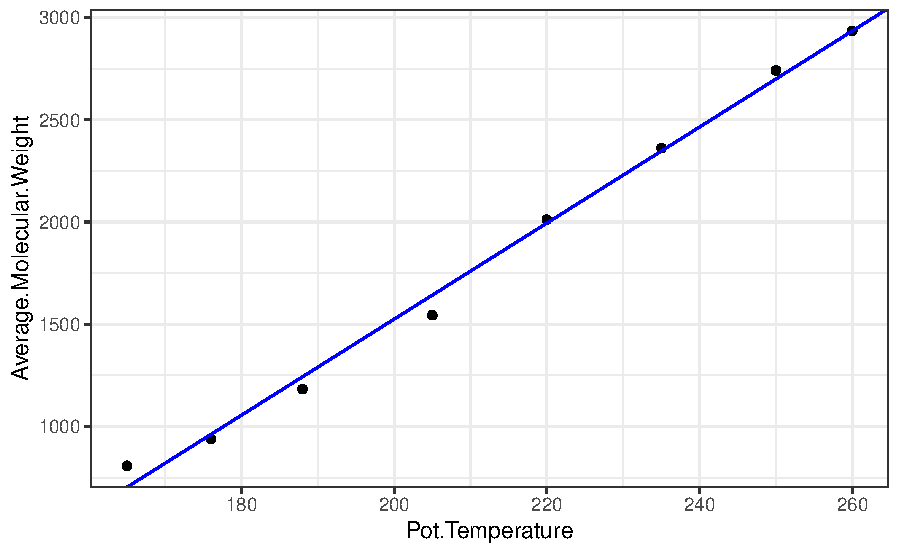
\includegraphics[width=0.6\textwidth]{figure/unnamed-chunk-3-1} 

}



\end{knitrout}
  \item (2 points)
  
  The residuals are: 105.355, -21.126, -60.105, -97.575, 16.951, 14.477, 42.003, 0.02.
  
\begin{knitrout}
\definecolor{shadecolor}{rgb}{0.969, 0.969, 0.969}\color{fgcolor}

{\centering 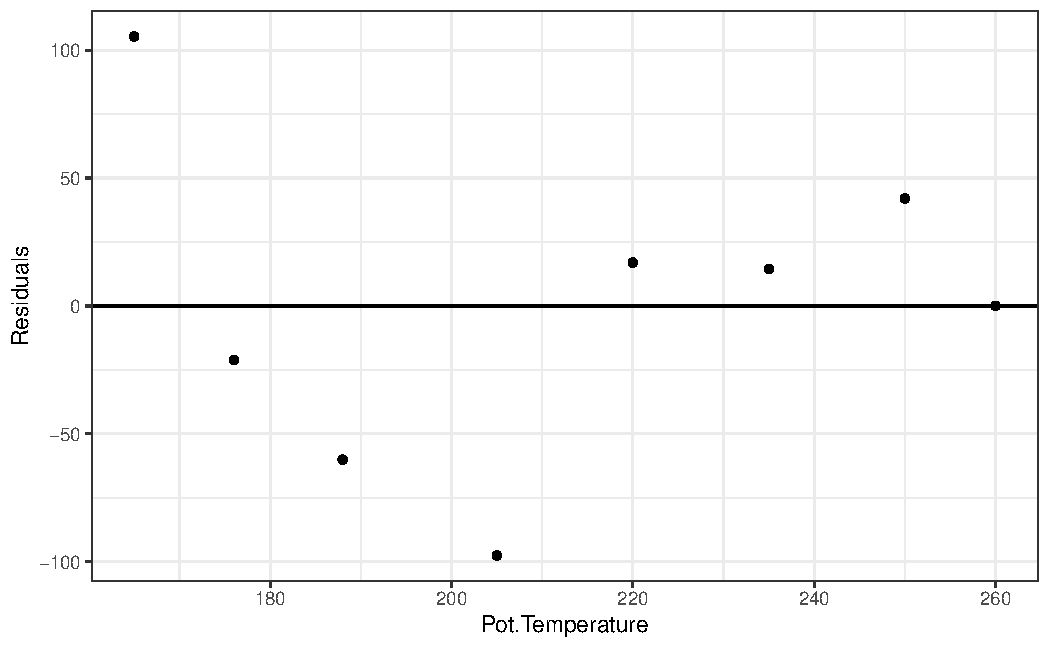
\includegraphics[width=0.6\textwidth]{figure/unnamed-chunk-4-1} 

}




{\centering 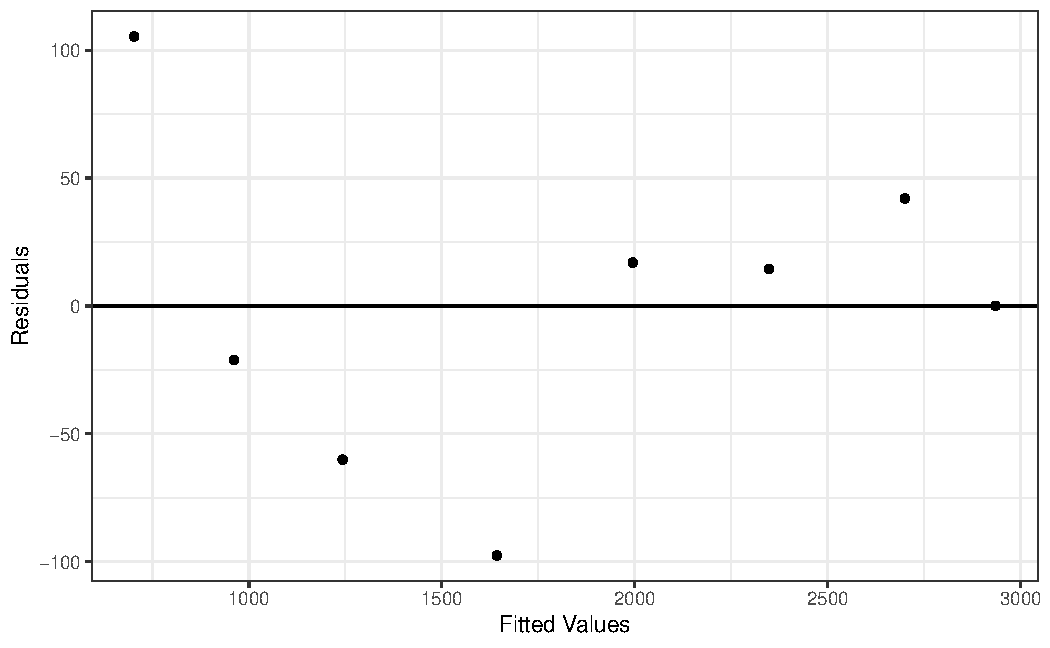
\includegraphics[width=0.6\textwidth]{figure/unnamed-chunk-4-2} 

}




{\centering 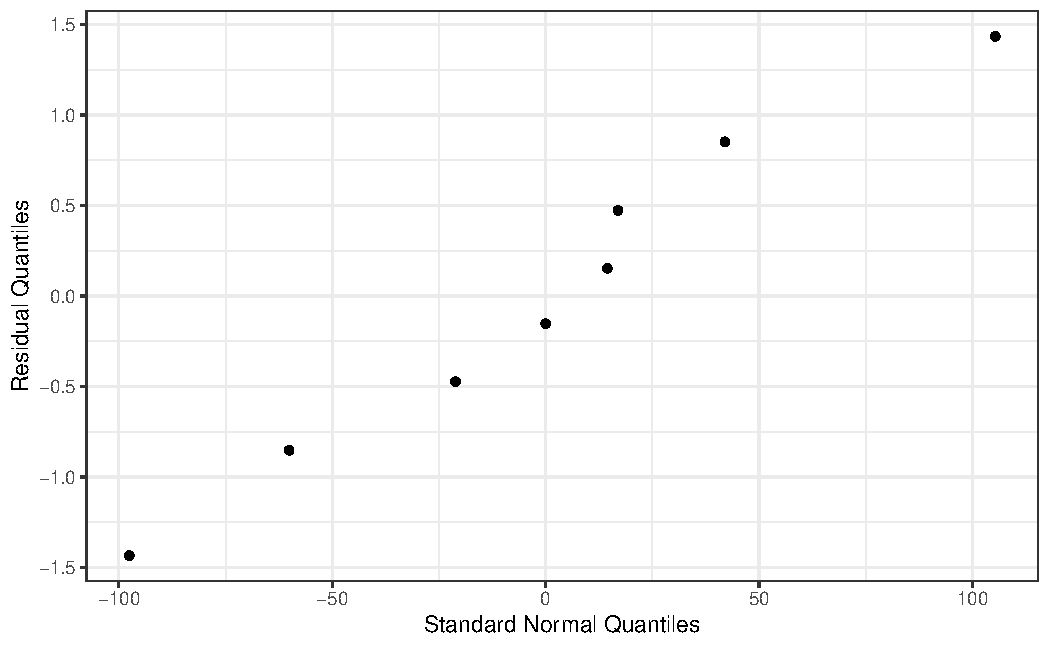
\includegraphics[width=0.6\textwidth]{figure/unnamed-chunk-4-3} 

}



\end{knitrout}
  
  It is difficult to evaluate the appropriateness of the fitted equation based on so little data. The plots of residuals versus $x$ and residuals versus $\hat{y}$ do not contain any obvious patterns, and thus provide no evidence that the equation is inappropriate. The normal plot of residuals is fairly linear, providing no evidence that the residuals are not bell-shaped.
  
\item (1 point)

There is no replication (multiple experimental runs at a particular pot temperature). Replication would validate any conclusions drawn from the experiment, and provide more information to confirm the appropriateness of the fitted equation.

\item (2 points)

For $x = \textrm{188\textdegree{C}}$,
\[\hat{y} = -3174.6 + 23.5(188) = 1243.1.\]

For $x = \textrm{200\textdegree{C}}$,
\[\hat{y} = -2174.6 + 23.5(200) = 1525.1.\]

It would not be wise to make a similar prediction at $x = \textrm{70\textdegree{C}}$ because there is no evidence that the fitted relationship is correct for pot temperature as low as $x = \textrm{70\textdegree{C}}$. This would be an extrapolation. Some data should be obtained around $x = \textrm{70\textdegree{C}}$ before making such a prediction.
  

	
	\end{enumerate}
	\item P. 161: 1 
	
		{\color{red}
	(9 points)
	
	The least squares equation is
	\[\hat{ y = -1315 + 5.59 x + .04212x^2}\]
	
\begin{knitrout}
\definecolor{shadecolor}{rgb}{0.969, 0.969, 0.969}\color{fgcolor}

{\centering 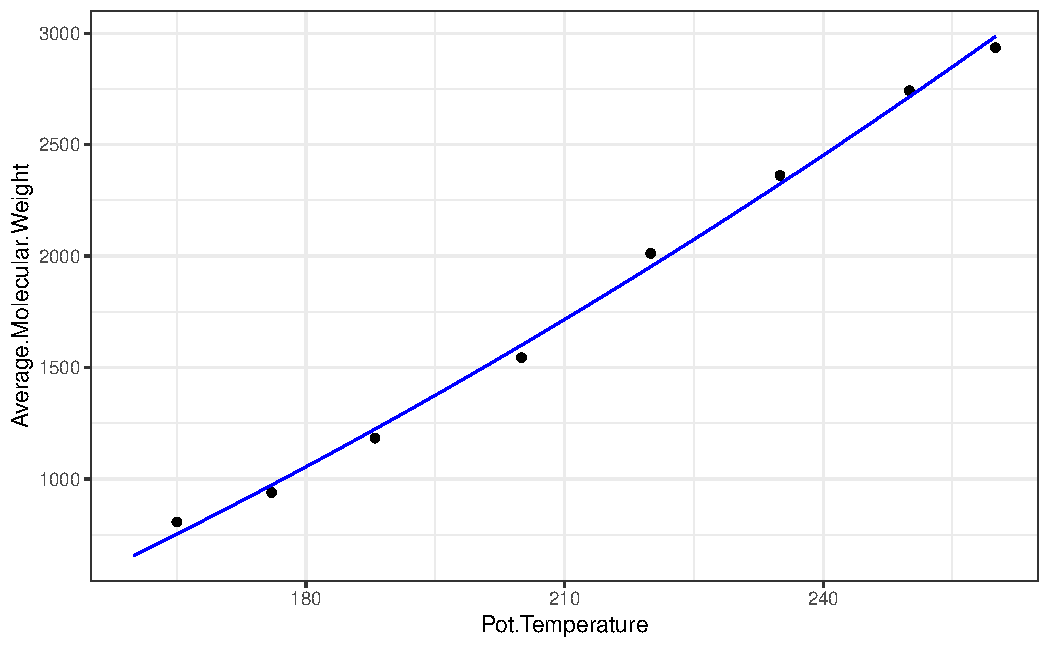
\includegraphics[width=0.6\textwidth]{figure/unnamed-chunk-5-1} 

}



\end{knitrout}
  
  $R^2_Q = .996$, compared with $R^2_L = .994$. This is a very small improvement, at a cost of a more complex equation.
  
\begin{knitrout}
\definecolor{shadecolor}{rgb}{0.969, 0.969, 0.969}\color{fgcolor}

{\centering 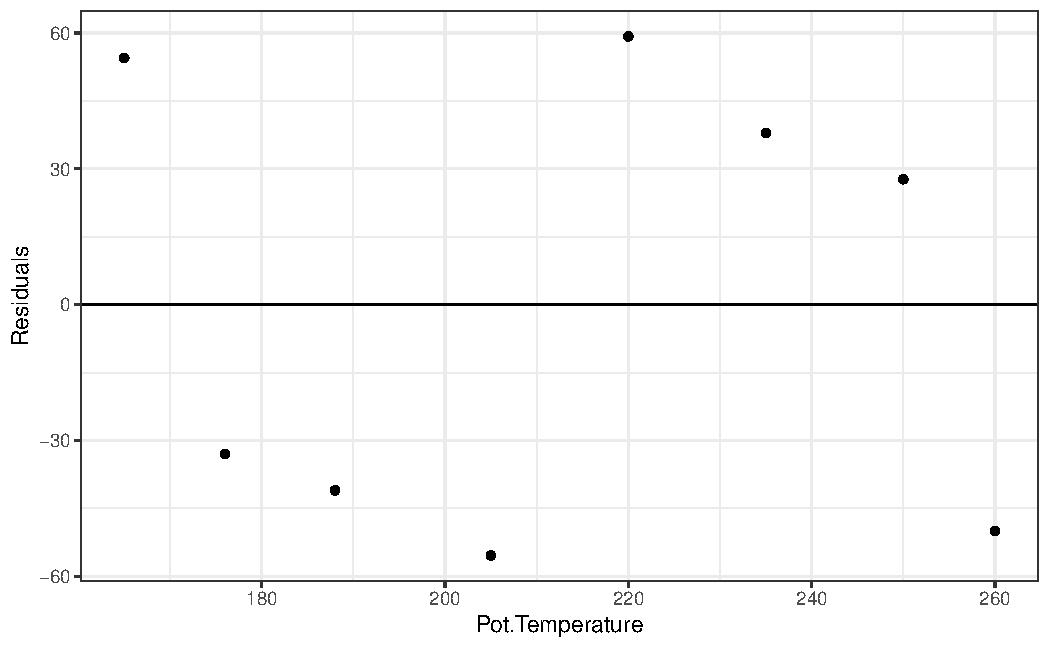
\includegraphics[width=0.6\textwidth]{figure/unnamed-chunk-6-1} 

}




{\centering 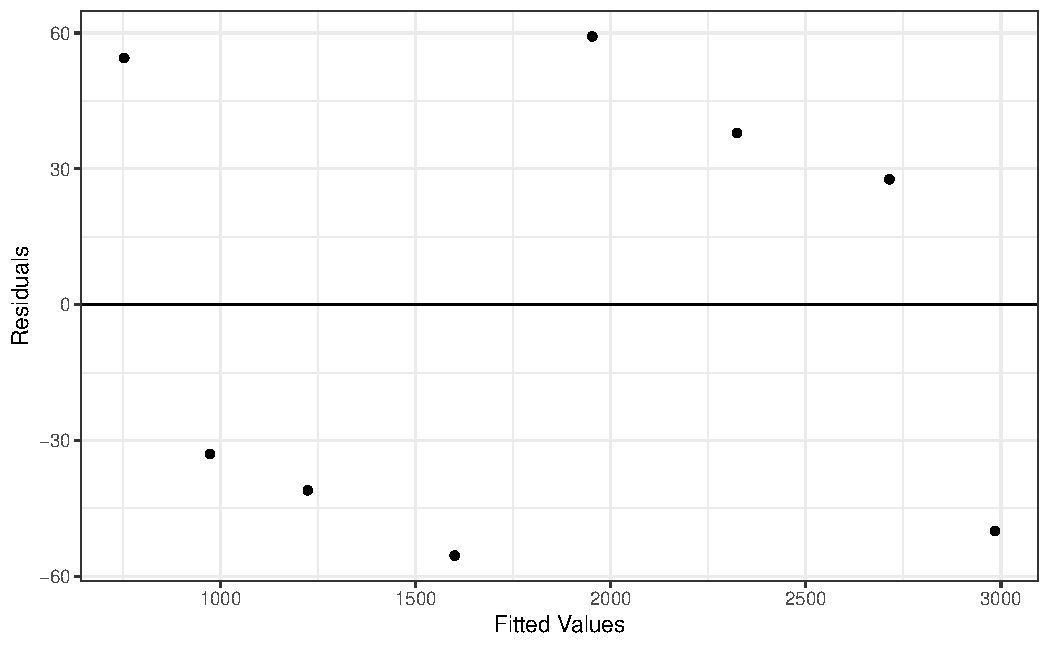
\includegraphics[width=0.6\textwidth]{figure/unnamed-chunk-6-2} 

}




{\centering 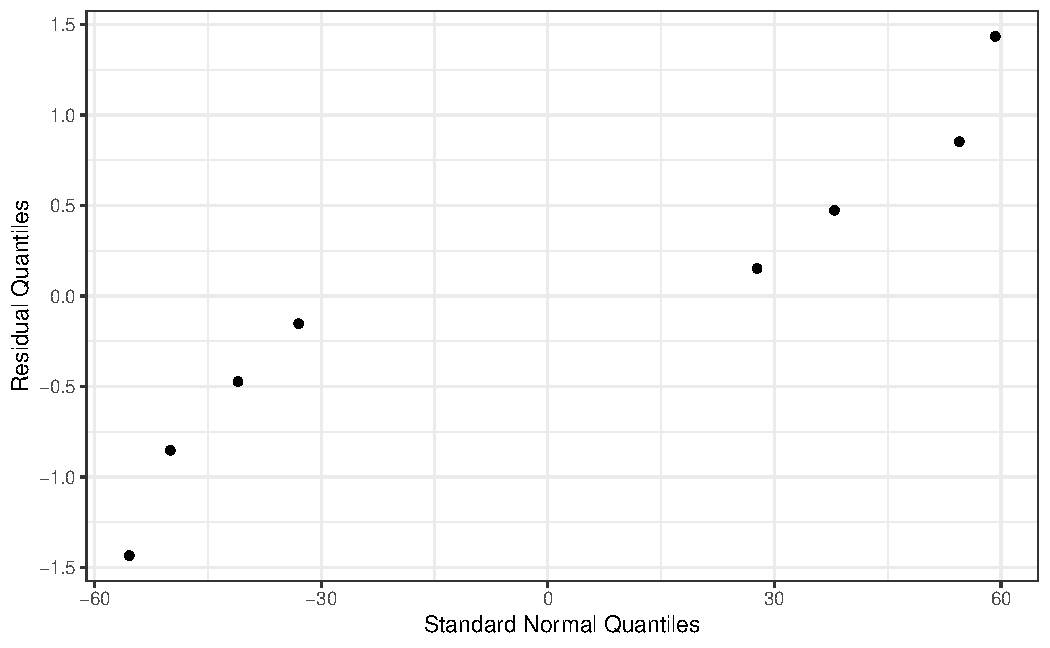
\includegraphics[width=0.6\textwidth]{figure/unnamed-chunk-6-3} 

}



\end{knitrout}
  
  The residuals here are smaller, as they will always be for a more complex model. There is no noticeable improvement in the residual plots, compared to those from the straight-line model. In fact, the residual plots for the quadratic model look more patterned. The scatterplot of $y$ versus $x$ also indicates that the quadratic model would be ``overfitting'' the data. The simpler straight-line relationship seems to be adequate.
  
  For the quadratic model, at $x = \textrm{200\textdegree{C}}$,
  \[ \hat{y} = -1315 + 5.59(200) + .04212(200)^2 = 1487.2,\]
  which is relatively close to 1525.1 from 4-5 (e).
  
	

	}
	
	\clearpage
	\item P. 140: 4 
	\begin{enumerate}
	\item (3 points)
	
\begin{knitrout}
\definecolor{shadecolor}{rgb}{0.969, 0.969, 0.969}\color{fgcolor}

{\centering 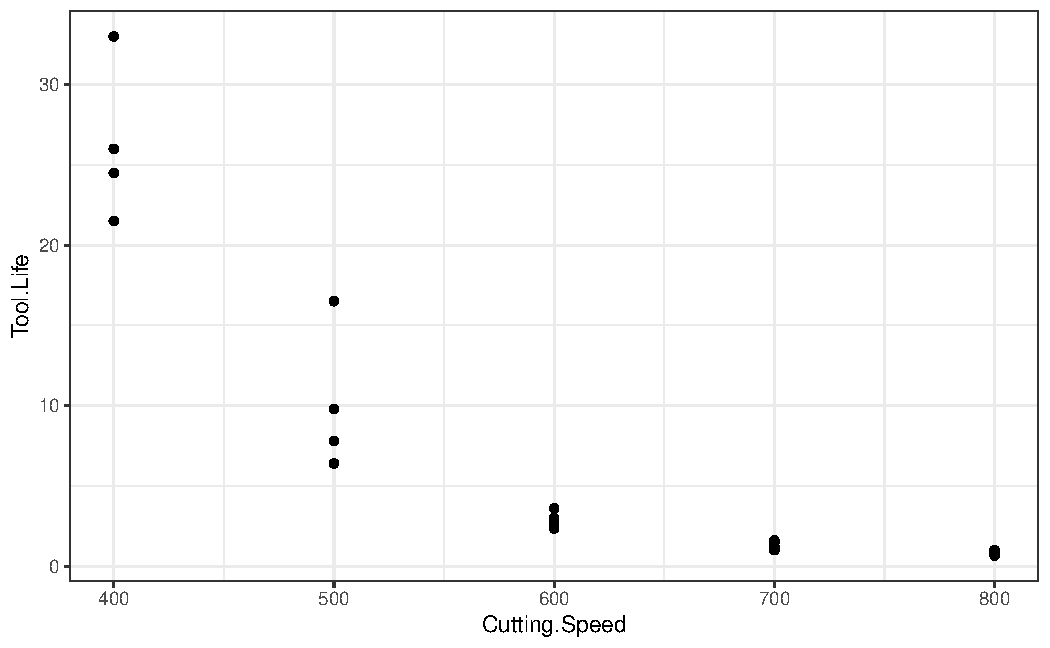
\includegraphics[width=0.6\textwidth]{figure/unnamed-chunk-7-1} 

}



\end{knitrout}
  
  The scatterplot is not linear, so the given straight-line relationship does not seem appropriate. The least squares line is $\hat{y} = 44.075 - .059650x$. The corresponding $R^2$ is .723.
  
  \item (3 points)
  
  \
  
  
\begin{knitrout}
\definecolor{shadecolor}{rgb}{0.969, 0.969, 0.969}\color{fgcolor}

{\centering 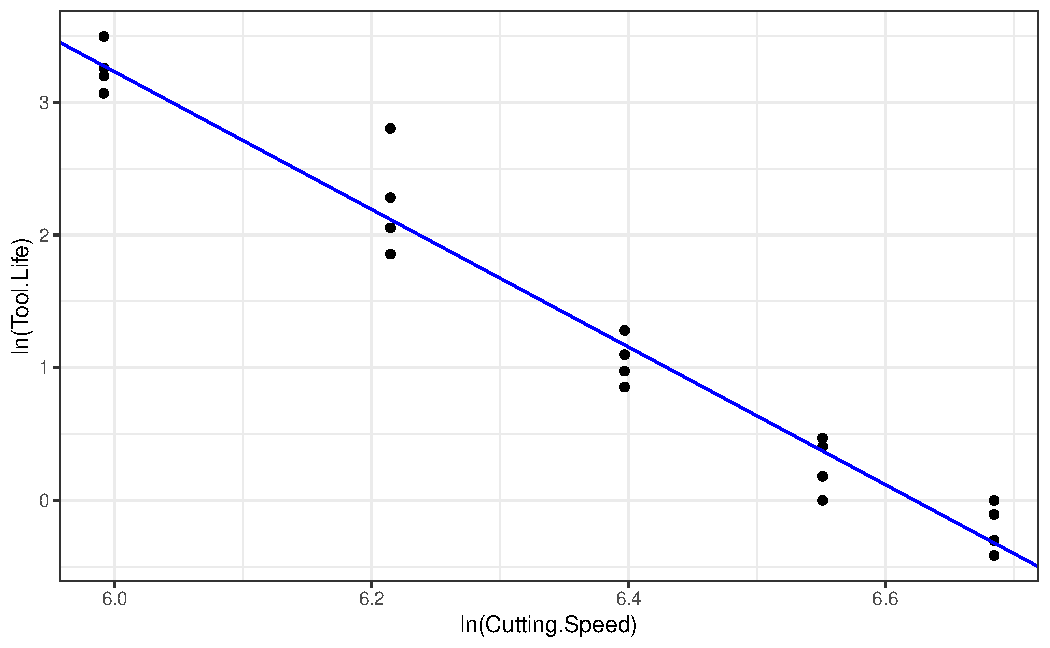
\includegraphics[width=0.6\textwidth]{figure/unnamed-chunk-8-1} 

}



\end{knitrout}
  
  This scatterplot is much more linear, and a straight-line relationship seems appropriate for the transformed variables. The least squares line is \[\widehat{\ln y} = 24.244 - 5.1857 \ln x.\] The corresponding $R^2$ is .965.
  
  \item (3 points)
  
  The least squares line is given in part (b). For $x = 550$,
  \[\widehat{\ln y} = 34.344 - 5.1857\ln(550) = 1.6229\ln{\mathrm{minutes}},\]
  so $\hat{y} = e^{1.6229} = 5.07\, \mathrm{minutes}$. The implied relationship between $x$ and $y$ is 
  \begin{align*}
  &y \approx e^{\beta_0 + \beta_1 \ln x}\\
  &y \approx e^{\beta_0} e^{\ln x^{\beta_1}}\\
  &y \approx e^{\beta_0} x^{\beta_1}.
  \end{align*}
  With slight rearrangement, this is the same as Taylor's equation for tool life.
	\end{enumerate}
	
	\clearpage
	\item P. 161: 2 

  \begin{enumerate}
  \item (3 points)
  
  The least square equation is
  \[\hat{y} = 6.0483 + .14167x_1 - .016944x_2.\]
  Assuming the fitted equation is appropriate, this means that as $x_1$ increases by 1\% (holding $x_2$ constant), $y$ increases by roughly $.14167 \mathrm{cm}^3\mathrm{\slash g}$. As $x_2$ increases by 1 minute (holding $x_1$ constant), $y$ decreases by roughly $.016944\mathrm{cm}^3\mathrm{\slash g}$. The $R^2$ corresponding to this equation is .807.
  
  \item (3 points)
  
  The residuals are -0.015, 0.143, 0.492, -0.595, -0.457, -0.188, 0.695, 0.143, -0.218.
  
\begin{knitrout}
\definecolor{shadecolor}{rgb}{0.969, 0.969, 0.969}\color{fgcolor}

{\centering 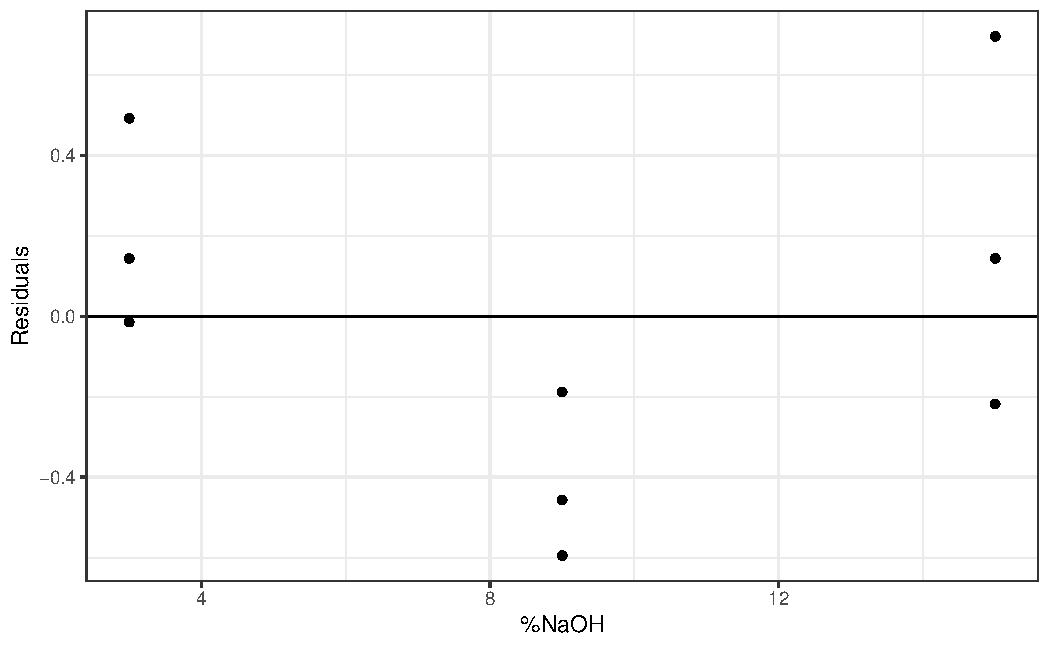
\includegraphics[width=.49\linewidth]{figure/fig-sub-1} 
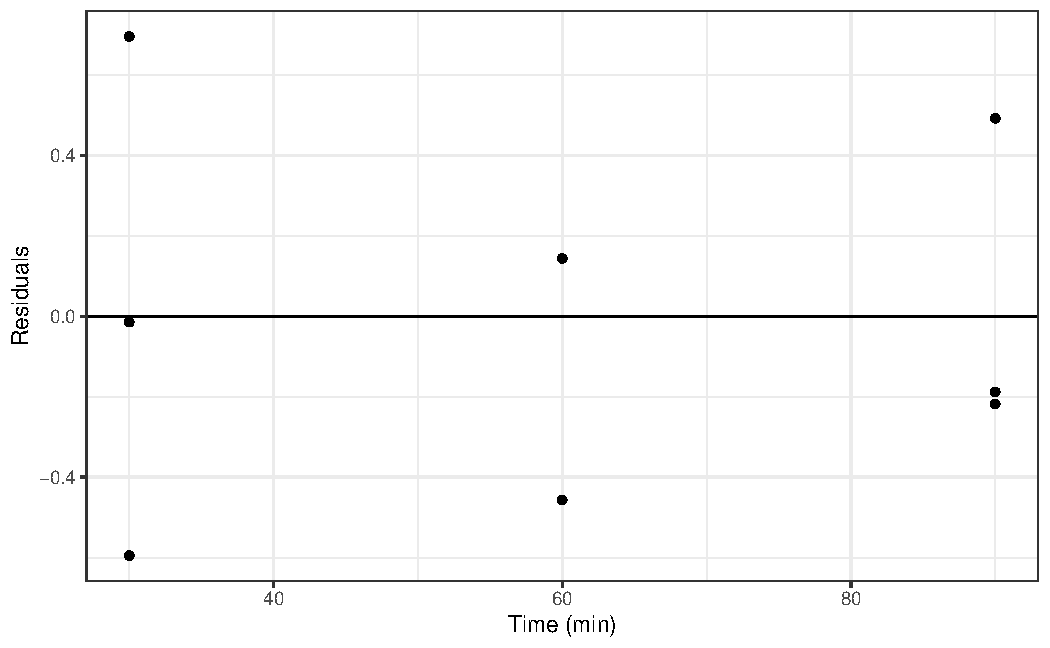
\includegraphics[width=.49\linewidth]{figure/fig-sub-2} 
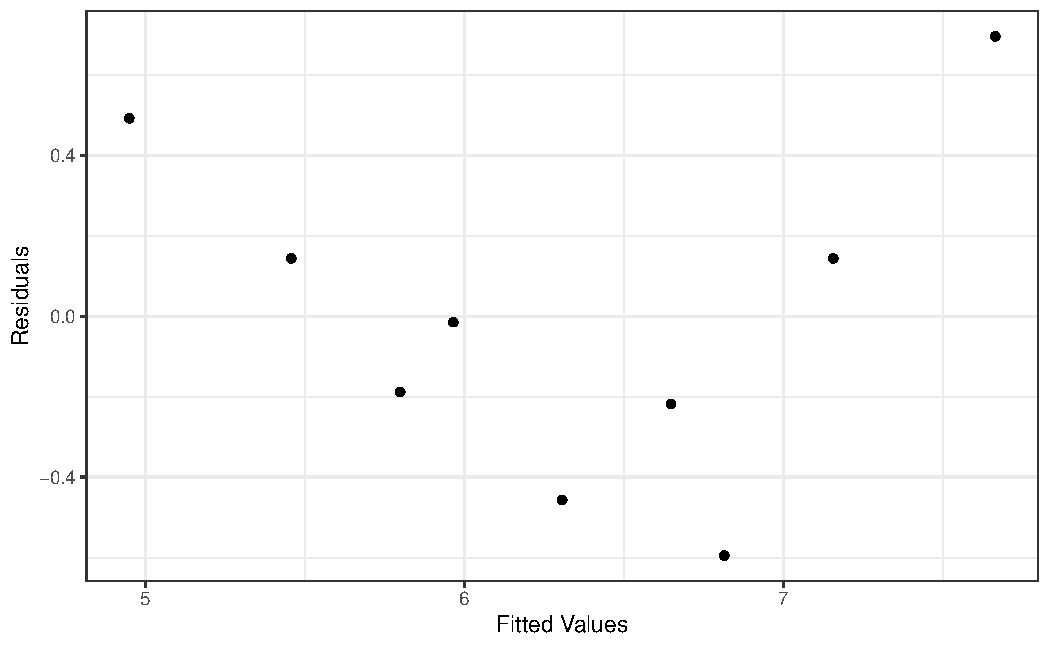
\includegraphics[width=.49\linewidth]{figure/fig-sub-3} 
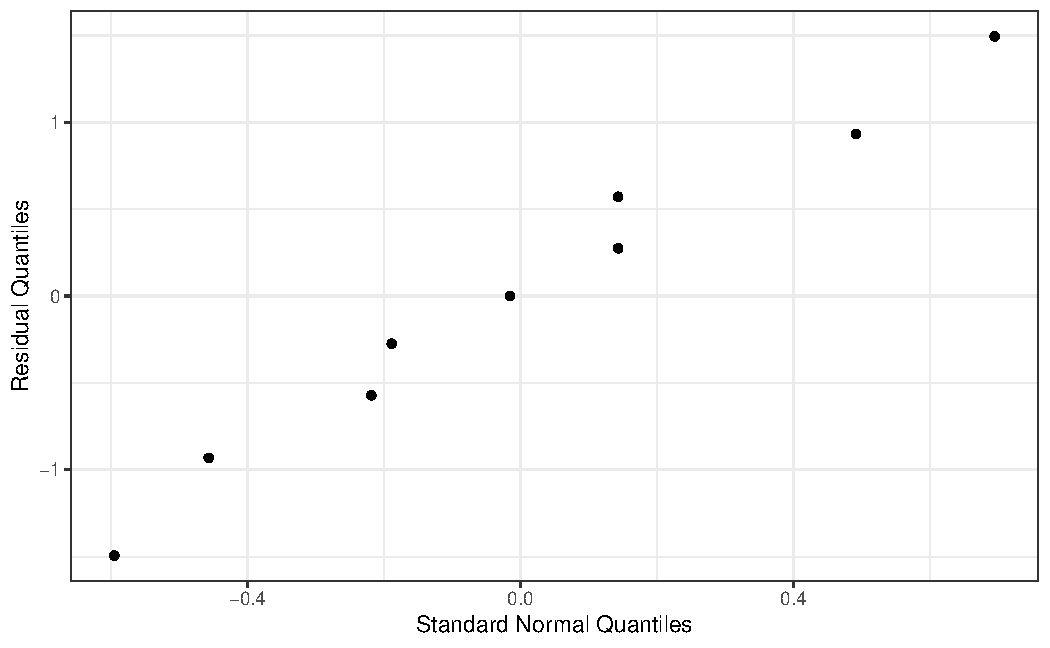
\includegraphics[width=.49\linewidth]{figure/fig-sub-4} 

}



\end{knitrout}
  
  Both the plots of residuals versus $x_1$ and residuals versus $\hat{y}$ show a positive-negative-positive pattern of residuals, indicating that the relationship between $x_1$ and $y$ is not completely accounted for by the current model. These plots suggest adding an $x_1^2$ term. The plot of residuals versus $x_2$ is patternless; $x_2$ seems to be well represented. The normal plot of residuals is fairly linear, indicating that the residuals are bell-shaped.
  
  \item (3 points)
  
  For $x_2 = 30$, the equation is
  \begin{align*}
  \hat{y} &= 6.0483 + .14167 x_1 - .016944(30) \\
  & = 5.53998 + .14167 x_1.
  \end{align*}
  
  For $x_2 = 60$, the equation is
  \begin{align*}
  \hat{y} &= 6.0483 + .14167 x_1 - .016944(60) \\
  & = 5.03166 + .14167 x_1.
  \end{align*}
  
  For $x_2 = 90$, the equation is
  \begin{align*}
  \hat{y} &= 6.0483 + .14167 x_1 - .016944(90) \\
  & = 4.52334 + .14167 x_1.
  \end{align*}
  
\begin{knitrout}
\definecolor{shadecolor}{rgb}{0.969, 0.969, 0.969}\color{fgcolor}

{\centering 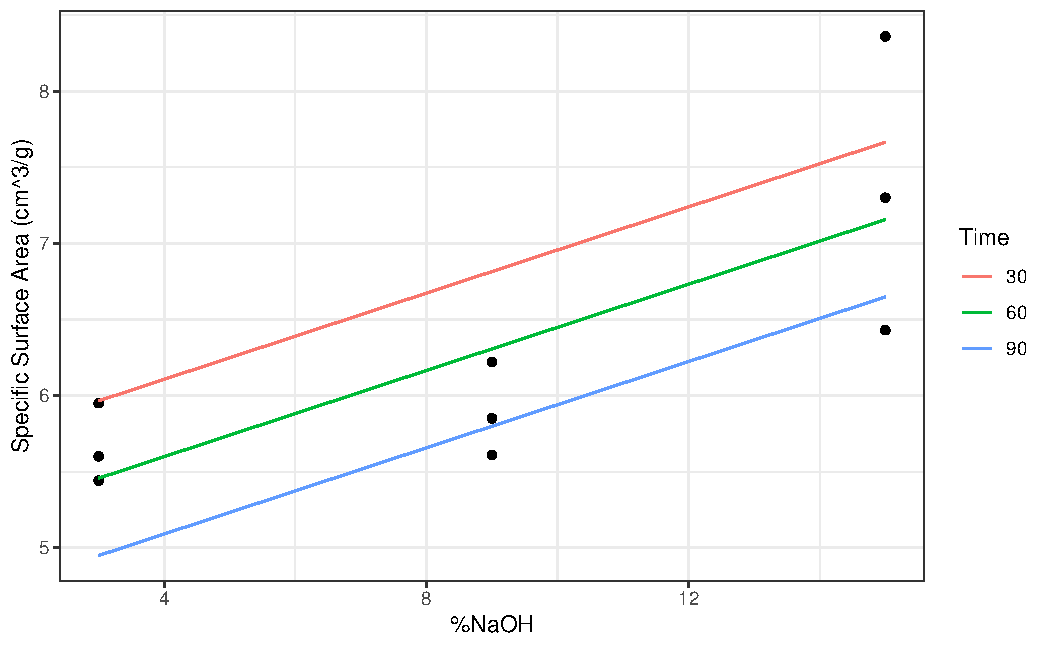
\includegraphics[width=0.6\textwidth]{figure/unnamed-chunk-10-1} 

}



\end{knitrout}
  
  The fitted responses do not match up well, because the relationship between $y$ and $x_1$ (\%NaOH) is not linear for any of the $x_2$ values (Time).
  
  \item (3 points)
  At $x_1 = 10\%$ and $x_2 = 70\mathrm{minutes}$,
  \[\hat{y} = 6.0483 + .14167(10) - .016944(70) = 6.279\mathrm{\,cm}^3\mathrm{\slash g}.\]
  
  It would not be wise to make a similar prediction at $x_1 = 10\%$ and $x_2 = 120 \mathrm{\,minutes}$ because there is no evidence that the fitted relationship is correct under these conditions. This would be extrapolating. Some data should be obtained around $x_1 = 10\%$ and $x_2 = 120 \mathrm{\,minutes}$ before making such a prediction.
  
  \item (3 points)
  The least squares equation is
  \[\hat{y} = 4.9833 + .260 x_1 + .00081 x_2 - .001972 x_1 x_2,\]
  and the corresponding $R^2$ is .876. The increase in $R^2$ from .807 to .876 is not very large; using the more complicated equation may not be desirable (this is subjective). Residual plots for this more complicated equation should also be examined before evaluating its appropriateness.
  
  \item (3 points)
  
  For $x_2 = 30$, the equation is
  \begin{align*}
  \hat{y} &= 4.9833 + .260 x_1 + .00081(30) - .001972 x_1 (30)\\
  &= 5.0076 + .20084 x_1.
  \end{align*}
  
  For $x_2 = 60$, the equation is
  \begin{align*}
  \hat{y} &= 4.9833 + .260 x_1 + .00081(60) - .001972 x_1 (60)\\
  &= 5.0319 + .14168 x_1.
  \end{align*}
  
  For $x_2 = 90$, the equation is
  \begin{align*}
  \hat{y} &= 4.9833 + .260 x_1 + .00081(30) - .001972 x_1 (30)\\
  &= 5.0562 + .08252 x_1.
  \end{align*}
  
\begin{knitrout}
\definecolor{shadecolor}{rgb}{0.969, 0.969, 0.969}\color{fgcolor}

{\centering 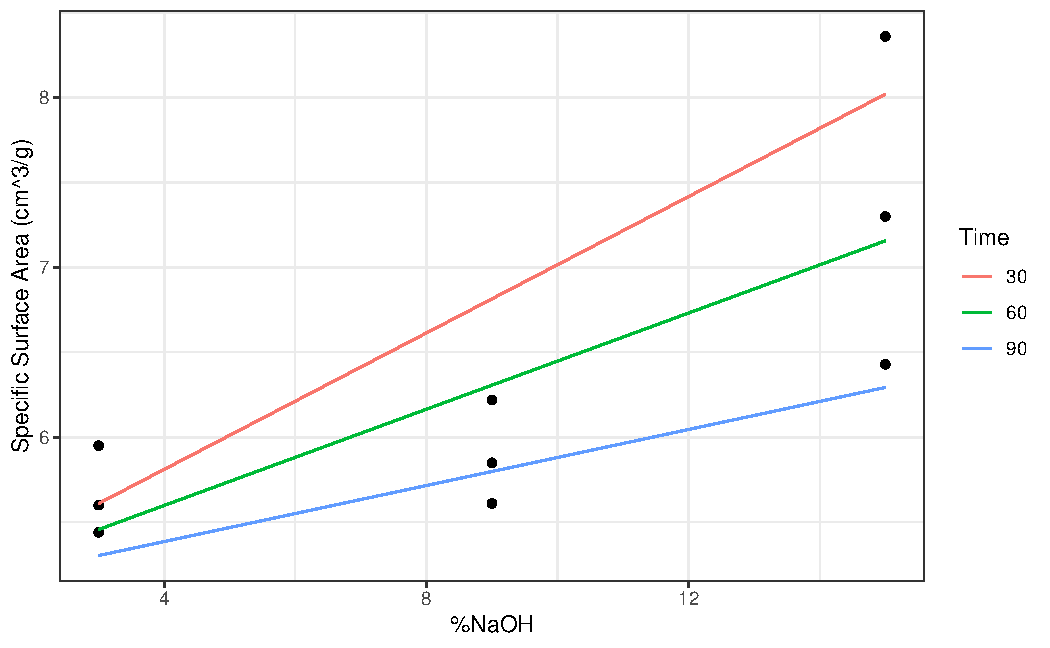
\includegraphics[width=0.6\textwidth]{figure/unnamed-chunk-11-1} 

}



\end{knitrout}
  
  The new model allows there to be a different slope for different values of $x_2$, so these lines fit the data better than the lines in part (c). But they still do not account for the non-linearity between $x_1$ and $y$. And equation with an $x_1^2$ term would fit much better.
  
  \item (3 points) There is no replication (multiple experimental runs at a particular NaOH-Time combination). Replication would validate any conclusions drawn from the experiment, and it would allow for better comparisons among the different possible fitted equations.
  
  \item (3 points)
  This data has a complete (full) factorial structure. The straight-line least squares equation for $x_1$ is 
  \[\hat{y} = 5.0317 + .14167 x_1\]
  with a corresponding $R^2$ of .594. The straight-line least squares equation for $x_2$ is
  \[\hat{y} = 7.3233 - .01694 x_2\]
  with a corresponding $R^2$ of .212. The slopes in these one-variable linear equations are the same as the corresponding slopes in the two-variable equation from (a). The $R^2$ value in (a) is the sum of the $R^2$ values from the two one-variable linear equations.
  \end{enumerate}
\end{enumerate}
%\newpage 
%\nocite{*}
%\bibliographystyle{plainnat} 
%\bibliography{}
\end{document}
